\documentclass{llncs}
\sloppy

%%%%%%%%%%%%%%%%%%%%%%%%%%%%%%%%%%%%%%%%%%%%%%%%%%%%%%%%%%%%
% PACKAGES
%%%%%%%%%%%%%%%%%%%%%%%%%%%%%%%%%%%%%%%%%%%%%%%%%%%%%%%%%%%%
\usepackage[utf8x]{inputenc}

% SYMBOLES
\usepackage{amsmath, amssymb, url} % amsthm, 

% ALGORITHMES
\usepackage[ruled,vlined,linesnumbered]{algorithm2e}



%%%%%%%%%%%%%%%%%%%%%%%%%%%%%%%%%%%%%%%%%%%%%%%%%%%%%%%%%%%%
% TIKZ
%%%%%%%%%%%%%%%%%%%%%%%%%%%%%%%%%%%%%%%%%%%%%%%%%%%%%%%%%%%%
\usepackage{pgf}
\usepackage{tikz}

\graphicspath{{./figures/}}

% Couleurs
\definecolor{turquoise}{rgb}{0 0.41 0.41}
\definecolor{rouge}{rgb}{0.79 0.0 0.1}
\definecolor{vert}{rgb}{0.15 0.4 0.1}
\definecolor{mauve}{rgb}{0.6 0.4 0.8}
\definecolor{violet}{rgb}{0.58 0. 0.41}
\definecolor{orange}{rgb}{0.8 0.4 0.2}
\definecolor{bleu}{rgb}{0.39, 0.58, 0.93}
\definecolor{gris}{rgb}{0.6,0.6,0.6}
\definecolor{grisfonce}{rgb}{0.4, 0.4, 0.4}
\definecolor{grispale}{rgb}{0.9, 0.9, 0.9}
% NOIR ET BLANC
\definecolor{vertfonce}{rgb}{0.0, 0, 0.0}
\definecolor{rougefonce}{rgb}{0, 0.0, 0.0}
\definecolor{rougeclair}{rgb}{0.6, 0.6, 0.6} %{red!50!white}
\definecolor{bleufonce}{rgb}{0.2, 0.2, 0.2} %blue!80!black
\definecolor{bleutresfonce}{rgb}{0.1, 0.1, 0.1} %blue!50!black
% \definecolor{vertfonce}{rgb}{0.0, 0.5, 0.0}
% \definecolor{rougefonce}{rgb}{1, 0.0, 0.0}
% \definecolor{rougeclair}{rgb}{1, 0.5, 0.5} %{red!50!white}
% \definecolor{bleufonce}{rgb}{0, 0, 0.8} %blue!80!black
% \definecolor{bleutresfonce}{rgb}{0, 0, 0.5} %blue!50!black


% Jeu de couleurs pales
% NOIR ET BLANC
\definecolor{cpale1}{rgb}{0.6, 0.6, 0.6}
\definecolor{cpale2}{rgb}{0.9, 0.9, 0.9}
% \definecolor{cpale1}{rgb}{1, 0.6, 0.6}
% \definecolor{cpale2}{rgb}{0.6, 1, 0.6}
\definecolor{cpale3}{rgb}{0.6, 0.6, 1}
\definecolor{cpale4}{rgb}{1, 0.6, 1}
\definecolor{cpale5}{rgb}{1, 1, 0.6}
\definecolor{cpale6}{rgb}{0.6, 1, 1}
\definecolor{cpale7}{rgb}{0.95, 0.65, 0.25}
\definecolor{cpale8}{rgb}{0.75, 0.45, 1}
\definecolor{cpale9}{rgb}{0.5, 1, 0.75}
\definecolor{cpale10}{rgb}{0.8, 0.7, 0.6}
\definecolor{cpale11}{rgb}{0.6, 0.7, 0.8}
\definecolor{cpale12}{rgb}{0.2, 0.5, 0.9}
\definecolor{cpale13}{rgb}{0.5, 0.9, 0.2}
\definecolor{cpale14}{rgb}{0.9, 0.2, 0.5}
\definecolor{cpale15}{rgb}{0.7, 0.7, 0.7}
\definecolor{cpale16}{rgb}{0.8, 0.8, 0.5}



%%%%%%%%%%%%%%%%%%%%%%%%%%%%%%%%%%%%%%%%%%%%%%%%%%%%%%%%%%%%
% CONSTANTES
%%%%%%%%%%%%%%%%%%%%%%%%%%%%%%%%%%%%%%%%%%%%%%%%%%%%%%%%%%%%

%-%-%-%-%-%-%-%-%-%-%-%-%-%-%-%-%-%-%-%-%-%-%-%-%-%-%-%-%-%
% CONSTANTES MATHEMATIQUES
%-%-%-%-%-%-%-%-%-%-%-%-%-%-%-%-%-%-%-%-%-%-%-%-%-%-%-%-%-%
% Booleens
\newcommand{\false}{{\tt false}}
\newcommand{\true}{{\tt true}}

% Ensembles
\newcommand{\AP}{\mathit{AP}}
\newcommand{\grandn}{{\mathbb N}}
\newcommand{\grandq}{{\mathbb Q}}
\newcommand{\grandqplus}{{\mathbb Q}_{\geq 0}}
\newcommand{\grandr}{{\mathbb R}}
\newcommand{\grandrplus}{\grandr_{\geq 0}}
\newcommand{\grandz}{{\mathbb Z}}
\newcommand{\setX}{\mathcal{K}_{\Clock}}
\newcommand{\setP}{\mathcal{K}_{\Param}}
\newcommand{\setXP}{\mathcal{K}_{\Clock \cup \Param}}

% Matrices
\newcommand{\matrixzero}{\mathbf{0}}
\newcommand{\matrixnopath}{\emptyset}

% Noms
\newcommand{\tiling}{\mathit{Tiling}}
\newcommand{\post}{\mathit{Post}}
\newcommand{\Pre}{\mathit{Pre}}
\newcommand{\TS}{\mathit{TS}}
\newcommand{\words}{\mathit{Words}}

% Operateurs
\DeclareMathOperator*{\argmax}{arg\,max}
\DeclareMathOperator*{\argmin}{arg\,min}
\newcommand{\eqdef}{ \overset{\mathit{def}}{=}}


% Symboles
\newcommand{\cro}[1]{\langle #1 \rangle}
\newcommand{\fleche}[1]{\stackrel{#1}{\rightarrow}}
\newcommand{\Fleche}[1]{\stackrel{#1}{\Rightarrow}}
\newcommand{\prefix}[2]{ |#1|_{#2} }
\newcommand{\steps}[0]{ {\rightarrow} }
\newcommand{\Steps}[0]{ {\Rightarrow} }
\newcommand{\timelaps}[1]{#1^\uparrow}
\newcommand{\trace}[1]{ \mathbin{<}#1 \mathbin{>}}
\newcommand{\wpi}[1]{\mathbin{<}#1\mathbin{>}}

% Temporal logics
\newcommand{\tlAlways}{\Box}
\newcommand{\tlEvt}{\Diamond}
\newcommand{\tlExists}{\exists}
\newcommand{\tlForall}{\forall}
\newcommand{\tlNext}{\bigcirc} % X
% \newcommand{\tlNext}{\circle}
\newcommand{\tlUntil}{\cup}

% Unites
\newcommand{\micros}{\mathit{\mu\,s}}
\newcommand{\millis}{\mathit{m\,s}}
\newcommand{\nanos}{ns}
\newcommand{\picos}{ps}


% Variables
\newcommand{\A}{\mathcal{A}}
\newcommand{\Avar}{\A_\mathit{var}}
\newcommand{\Clock}{X} % set of clocks
\newcommand{\clock}{x} % clock
\newcommand{\clockval}{w} % clock valuation
\newcommand{\enabled}{\mathit{enabled}}
\newcommand{\events}{E} % a possible set of events
\newcommand{\EventsSet}{\Sigma} % all possible events
\newcommand{\formule}{\varphi}
\newcommand{\Formule}{\Phi}
% \newcommand{\Kinit}{K_\mathit{init}} % initial constraint on the parameters
\newcommand{\LTS}{\mathcal{L}}
\newcommand{\Param}{P} % set of parameters (P / Y)
\newcommand{\param}{p} % parameter (p / y)
\newcommand{\py}{\pi} % parameter valuation
\newcommand{\Py}{\Pi} % set of consistent parameter valuations
\newcommand{\sinit}{s_\mathit{init}} % initial set of states
\newcommand{\Slast}{S_\mathit{last}}



\newcommand{\Ko}{K}
\newcommand{\pio}{\pi_0}
\newcommand{\piprime}{\pi}
\newcommand{\To}{T_0}
\newcommand{\Tprime}{T}


% \newcommand{\compyes}{\textcolor{green}{yes}}
\newcommand{\compyes}{$\textcolor{vertfonce}{\mathbf{\surd}}$}
% \newcommand{\compno}{\textcolor{red}{no}}
\newcommand{\compno}{$\textcolor{rougefonce}{\mathbf{\times}}$}


% Pour MDP
\newcommand{\we}{w}
\newcommand{\We}{W}
\newcommand{\va}{v}
\newcommand{\Va}{V}
\newcommand{\prob}{\mathit{Prob}}

%-%-%-%-%-%-%-%-%-%-%-%-%-%-%-%-%-%-%-%-%-%-%-%-%-%-%-%-%-%
% PARAMETRES
%-%-%-%-%-%-%-%-%-%-%-%-%-%-%-%-%-%-%-%-%-%-%-%-%-%-%-%-%-%
% PARAMETRES BRP
\newcommand{\brpMAX}{\mathit{MAX}}
\newcommand{\brpSYNC}{\mathit{SYNC}}
\newcommand{\brpTD}{\mathit{TD}}
\newcommand{\brpTR}{\mathit{TR}}
\newcommand{\brpTun}{\mathit{T1}}

% PARAMETRES CSMACD
\newcommand{\slot}{\mathit{slot}}

% PARAMETRES FLIP FLOP
\newcommand{\THold}{T_{\mathit{Hold}}}
\newcommand{\TSetup}{T_{\mathit{Setup}}}
\newcommand{\THI}{T_{\mathit{HI}}}
\newcommand{\TLO}{T_{\mathit{LO}}}
\newcommand{\TCKQ}{T_{ \mathit{CK} \rightarrow Q}}

% PARAMETRES RCP
\newcommand{\rcpFMax}{\mathit{f\_max}} % \mathit{rc\_fast\_max}
\newcommand{\rcpFMin}{\mathit{f\_min}} % \mathit{rc\_fast\_min}
\newcommand{\rcpSMax}{\mathit{s\_max}} % \mathit{rc\_slow\_max}
\newcommand{\rcpSMin}{\mathit{s\_min}} % \mathit{rc\_slow\_min}
\newcommand{\rcpD}{\mathit{delay}}

% PARAMETRES SIMOP
\newcommand{\COMct}{\mathit{COMct}}
\newcommand{\COMd}{\mathit{COMd}}
\newcommand{\NETd}{\mathit{NETd}}
\newcommand{\PLCct}{\mathit{PLCct}}
\newcommand{\PLCmtt}{\mathit{PLCmtt}}
\newcommand{\RIOd}{\mathit{RIOd}}
\newcommand{\SIGmrt}{\mathit{SIGmrt}}

% PARAMETRES SPSMALL
\newcommand{\tSetupA}{t_\mathit{setup}^A}
\newcommand{\tSetupD}{t_\mathit{setup}^D}
\newcommand{\tSetupWen}{t_\mathit{setup}^\mathit{WEN}}


% PARAMETRES WLAN
\newcommand{\pACK}{\mathit{ACK}}
\newcommand{\pACKTO}{\mathit{ACKTO}}
\newcommand{\pASLOTTIME}{\mathit{ASLOTTIME}}
\newcommand{\pBOFF}{\mathit{BOFF}}
\newcommand{\pDIFS}{\mathit{DIFS}}
\newcommand{\pMAXCOL}{\mathit{MAXCOL}}
\newcommand{\pSIFS}{\mathit{SIFS}}
\newcommand{\pTRANSTIMEMIN}{\mathit{TTMIN}}
\newcommand{\pTRANSTIMEMAX}{\mathit{TTMAX}}
\newcommand{\pVULN}{\mathit{VULN}}


%-%-%-%-%-%-%-%-%-%-%-%-%-%-%-%-%-%-%-%-%-%-%-%-%-%-%-%-%-%
% ALGORITHMES
%-%-%-%-%-%-%-%-%-%-%-%-%-%-%-%-%-%-%-%-%-%-%-%-%-%-%-%-%-%
% Algorithmes PTA
\newcommand{\IM}{\mathit{IM}}
\newcommand{\IMincl}{\IM_\subseteq}
\newcommand{\IMK}{\IM^K}
\newcommand{\IMunion}{\IM^\cup}
\newcommand{\IMinclK}{\IM^K_\subseteq}
\newcommand{\IMinclunion}{\IM^\cup_\subseteq}
\newcommand{\IMotf}{\IM_\mathit{otf}}
\newcommand{\BC}{\mathit{BC}}
\newcommand{\BCincl}{\BC_\subseteq}
\newcommand{\BCK}{\BC^K}
\newcommand{\BCunion}{\BC^\cup}
\newcommand{\BCinclK}{\BC^K_\subseteq}
\newcommand{\BCinclunion}{\BC^\cup_\subseteq}


%-%-%-%-%-%-%-%-%-%-%-%-%-%-%-%-%-%-%-%-%-%-%-%-%-%-%-%-%-%
% CONSTANTES DE CHAINES
%-%-%-%-%-%-%-%-%-%-%-%-%-%-%-%-%-%-%-%-%-%-%-%-%-%-%-%-%-%

% Langue
\newcommand{\absurde}{\emph{reductio ad absurdum}}

% Divers (projets et technique)

\newcommand{\lipsix}{LIP\,6}
\newcommand{\parissix}{Universit\'e Pierre et Marie Curie}
\newcommand{\simop}{SIMOP}
\newcommand{\spsmall}{SPSMALL}
\newcommand{\stm}{ST-Microelectronics}
\newcommand{\therac}{Therac-25}
\newcommand{\valmem}{VALMEM}

% Outils
\newcommand{\apron}{\textsc{Apron}}
\newcommand{\gdot}{\textsc{dot}}
\newcommand{\graphviz}{Graphviz}
\newcommand{\hytech}{{\sc HyTech}}
\newcommand{\imitator}{\textsc{Imitator}}
\newcommand{\imitatordeux}{\textsc{Imitator}\,II}
% \newcommand{\hymitator}{\textsc{Hymitator}}
\newcommand{\kronos}{\textsc{Kronos}}
\newcommand{\nusmv}{NuSMV}
\newcommand{\ocaml}{OCaml}
\newcommand{\phaver}{PHAVer}
\newcommand{\plot}{gnuplot}
\newcommand{\polka}{NewPolka}
\newcommand{\prism}{\textsc{Prism}}
\newcommand{\python}{Python}
\newcommand{\red}{RED}
\newcommand{\romeo}{Rom\'eo}
\newcommand{\smv}{SMV}
\newcommand{\spin}{Spin}
\newcommand{\tina}{TINA}
\newcommand{\trex}{\textsc{TReX}}
\newcommand{\uppaal}{\textsc{Uppaal}}
\newcommand{\vhdlta}{\textsc{Vhdl2Ta}}






%%%%%%%%%%%%%%%%%%%%%%%%%%%%%%%%%%%%%%%%%%%%%%%%%%%%%%%%%%%%
% FORMATING
%%%%%%%%%%%%%%%%%%%%%%%%%%%%%%%%%%%%%%%%%%%%%%%%%%%%%%%%%%%%

% CODE INTEGRE AU TEXTE
\newcommand{\code}[1]{\textbf{\texttt{#1}}}

% COMMENTAIRE DANS UN ALGORITHME
\newcommand{\comalgo}[1]{\textcolor{grisfonce}{\tcp*{ #1 }}}


% COMMENTAIRES DANS UN PARAGRAPHE
\newcommand{\commentaire}[1]{\textcolor{red}{\textbf{$\Leftarrow$  #1 $\Rightarrow$}}}
% \newcommand{\commentaire}[1]{}

% REDEFINITIONS DES PARAGRAPHES
\newcommand{\paragraphe}[1]{\paragraph{#1.}}
% \newcommand{\paragraphe}[1]{\subsubsection{#1.}}


% Title
% \title{Parametric Scheduling with IMITATOR}
% \title{IMITATOR with Stopwatches and its Applications to Parametric Preemptive Scheduling}
\title{IMITATOR 2.5: A Tool for Analyzing Robustness in Scheduling Problems}
\author{\'Etienne Andr\'e$^1$, Laurent Fribourg$^2$, Ulrich K\"uhne$^3$ and Romain Soulat$^2$}
\institute{$^1$LIPN, CNRS UMR 7030, Université Paris 13, France \\
$^2$LSV -- ENS Cachan \& CNRS \\
$^3$Universit\"at Bremen, Germany}




\begin{document}

\maketitle

\begin{abstract}
% 	We present here \imitator{} 2.5.
	The tool \imitator{}  implements the {\em Inverse Method} ($\IM$) for Timed Automata (TAs).
	Given a TA~$\A$ and a tuple $\pio$ of reference valuations for timings,
	$\IM$ synthesizes a constraint around  $\pio$ where $\A$ behaves in the same discrete manner.
	This provides us with a quantitative measure of robustness of the behavior of $\A$ around $\pio$.
	The new version \imitator{} 2.5 integrates the new features of stopwatches (in addition to standard clocks) and updates (in addition to standard clock resets), as well as powerful algorithmic improvements for state space reduction.
	These new features make the tool well-suited to analyze the robustness of solutions in several classes of preemptive scheduling problems.
\end{abstract}

\keywords{%{\bf keywords:}
	Real-Time Systems, 
	%Preemptive Scheduling, 
	Parametric Timed Automata,
	Stopwatches
	%, Parameter Synthesis
}

%%%\commentaire{Version avec commentaires}

% (preemptive)



% 1) 
% % dessin (sans ppl)
% % parg2 sec 2
% % proprietes im (1) et (2)
% 
% 
% stopwatches: efficace pour robustesse scheduking
% motiv' rapport
% 
% 2) historique
% 
% 3) archi
% 
% 4) etudes de cas --> appendix
% 





%%%%%%%%%%%%%%%%%%%%%%%%%%%%%%%%%%%%%%%%%%%%%%%%%%%%%%%%%%%%
%%%%%%%%%%%%%%%%%%%%%%%%%%%%%%%%%%%%%%%%%%%%%%%%%%%%%%%%%%%%
\section{Motivation}
%%%%%%%%%%%%%%%%%%%%%%%%%%%%%%%%%%%%%%%%%%%%%%%%%%%%%%%%%%%%
%%%%%%%%%%%%%%%%%%%%%%%%%%%%%%%%%%%%%%%%%%%%%%%%%%%%%%%%%%%%

% The specification and verification of real-time systems, involving concurrency and timing delays, are notoriously difficult problems.
% The correctness of such real-time systems usually depends on the values of these timing delays.
% One can check the correctness for one particular value for each delay, but this does not guarantee the correctness for other values.
% Actually, checking the correctness for all possible delays, even in a bounded interval, would require an infinite number of calls to the model checker, because those delays can have real (or rational) values.
% It is therefore interesting to consider that these delays are \emph{parameters} (unknown constants), and synthesize a constraint on these parameters guaranteeing a correct behavior.


\imitator{} 2.5 (for \emph{Inverse Method for Inferring Time AbstracT behaviOR}) is a tool for parameter synthesis in the framework of real-time systems based on the inverse method~$\IM$ for Parametric Timed Automata (PTAs).  % ,~\cite{ad94}
Different from CEGAR-based methods% (see \cite{cgjlv00})
, this algorithm for parameter synthesis makes use of a ``good'' parameter valuation~$\pio$ instead of a set of ``bad'' states~\cite{acef09}.
\imitator{} takes as input a network of PTAs with stopwatches
and a reference valuation~$\pio$; it synthesizes a constraint~$\Ko$ on the parameters such that (1) $\pio \models \Ko$ and (2) for all parameter valuation~$\piprime$ satisfying $\Ko$, the trace set (i.e., the discrete behavior) of~$\A$ under~$\piprime$ is the same as for~$\A$ under~$\pio$.
%This preserves in particular linear time properties, 
This provides the system with a criterion of \emph{robustness} (see, e.g., \cite{m11})
%, by formally guaranteeing a uniform discrete behavior 
around~$\pio$.

% It , that synchronize on shared actions
% The input syntax, inspired by~\hytech{}, allows the use of clocks (or stopwatches), rational-valued discrete variables, and parameters (i.e. unknown constants) to be used altogether in linear terms, within guards, invariants and updates.

% By iterating the inverse method on all integer points within a bounded reference parameter domain, we get a set of constraints %(``tiles'')
% such that, for every point in each such constraint, the time-abstract behavior is the same: this gives a behavioral cartography of the system~\cite{af10}.



%-%-%-%-%-%-%-%-%-%-%-%-%-%-%-%-%-%-%-%-%-%-%-%-%-%-%-%-%-%-%
\begin{figure}[ht!]
	% STYLES
	\tikzstyle{etiquette} = [draw=none, color=black]
	
% \tikzstyle{boite}=[text width=8em, text centered, minimum height=2.5em, rounded corners, very thick]
% \tikzstyle{input}=[boite, draw=green!20!gris, top color=green!50, bottom color=green!10!white]
% \tikzstyle{output}=[boite, draw=red!20!gris, top color=red!50, bottom color=red!5!white]
% \tikzstyle{imitator} = [boite, draw=blue!20!gris, text width=10em, minimum height=6em]

	
	\tikzstyle{boite}=[rectangle, draw=black, rounded corners, thick, draw=blue!40!black, top color=blue!20, bottom color=blue!5!white]
% 	\tikzstyle{imitator} = [boite]
% 	\tikzstyle{apron} = [boite, draw=yellow!20!gris, top color=yellow!70, bottom color=yellow!10!white]
% 	\tikzstyle{polka} = [apron]
% 	\tikzstyle{ppl} = [apron]
	\tikzstyle{dot} = [boite, draw=purple!20!gris, top color=purple!60, bottom color=purple!10!white]

	\tikzstyle{fleche} = [->, draw=black, semithick]
{

\centering

\begin{tikzpicture}[scale=0.6,  =>stealth']

	% Boites
	\draw[boite] (-5, 5.5) rectangle (-2, 6.5);
	\node [etiquette] at (-3.5, 6) {PTA};
	
	\draw[boite] (-5, 3.8) rectangle (-2, 5);
	\node [etiquette] at (-3.5, 4.4) {\begin{tabular}{c}Reference\\valuation $\pio$\end{tabular}};
	
	\draw[boite] (0, 4) rectangle (6, 6.5);
	\node [etiquette] at (3, 5.25) {\large \imitator{}};
	
% 	\draw[boite] (1, 4) rectangle (5, 5);
% 	\node [etiquette] at (3, 4.5) {PPL};
	
	\draw[boite] (8, 4.5) rectangle (12, 6);
	\node [etiquette] at (10, 5.25) {Constraint $\Ko$};
	
% 	\draw[boite] (8, 4) rectangle (12, 5);
% 	\node [etiquette] at (10, 4.5) {Trace set};

	% Fleches
	\path[fleche] (-2, 6) --++ (2, 0);
	\path[fleche] (-2, 4.4) --++ (2, 0);
% 	\path[fleche] (3.5, 4) --++ (0, -.5);
% 	\path[fleche] (2.5, 3.5) --++ (0, .5);
	\path[fleche] (6, 5.25) --++ (2, 0);
% 	\path[fleche] (6, 4.5) --++ (2, 0);

\end{tikzpicture}

}

\caption{Functional view of \imitator{}}
\label{fig:structure}
\end{figure}
%-%-%-%-%-%-%-%-%-%-%-%-%-%-%-%-%-%-%-%-%-%-%-%-%-%-%-%-%-%-%


%%%%%%%%%%%%%%%%%%%%%%%%%%%%%%%%%%%%%%%%%%%%%%%%%%%%%%%%%%%%
\subsubsection*{History and New Features}
%%%%%%%%%%%%%%%%%%%%%%%%%%%%%%%%%%%%%%%%%%%%%%%%%%%%%%%%%%%%

A basic implementation named \imitator{} has first been proposed%in~\cite{and09}
, under the form of a \python{} script calling \hytech{}~\cite{hhw97}.
The tool has then been entirely rewritten in \imitatordeux{}~\cite{and10}, under the form of a standalone \ocaml{} program.
% able to verify a number of parametric case studies. % making use of the Parma Polyhedra Library (PPL)~\cite{bhz08}.
A number of case studies containing up to 60 timing parameters could be efficiently verified in the purely timed framework.

Since~\cite{and10}, we extended the input formalism to PTAs equipped with \emph{stopwatches}: clocks can now be stopped for some time while others keep growing.
Also, we added clock updates: clocks can now be set to arbitrary linear combinations of other clocks, parameters
and discrete variables.
% We also implemented further algorithms based on~$\IM$, that satisfy weaker properties than the preservation of the trace sets, while outputting larger sets of parameter valuations than~$\IM$ (and possibly non-convex).
These extensions, together with powerful algorithmic improvements for state space reduction, allow us to consider larger classes of case studies, 
such as scheduling problems.

% \commentaire{Laurent a dit :
% - le principe de la methode inverse pour les TA a été implémenté de façon basique ([ICTAC09])
% puis de façon sophistiquée ([Infinity10])\\
% - la méthode a été étendue pour les HA et implémentée de façon basique ([RP11])\\
% - il s'agit "ici" de décrire une implémentation sophistiquée (intégrant notamment des extensions
% du merging des TA  à la  [NFM 12] aux HA)
% }

%%%%%%%%%%%%%%%%%%%%%%%%%%%%%%%%%%%%%%%%%%%%%%%%%%%%%%%%%%%%
%%%%%%%%%%%%%%%%%%%%%%%%%%%%%%%%%%%%%%%%%%%%%%%%%%%%%%%%%%%%
\section{Architecture and Features}
%%%%%%%%%%%%%%%%%%%%%%%%%%%%%%%%%%%%%%%%%%%%%%%%%%%%%%%%%%%%
%%%%%%%%%%%%%%%%%%%%%%%%%%%%%%%%%%%%%%%%%%%%%%%%%%%%%%%%%%%%

The core of \imitator{} (available under the GNU GPL license) is written in OCaml, and interacts with the Parma Polyhedra Library (PPL)~\cite{bhz08}.
Exact arithmetics with unbounded precision is used.
% 
\imitator{} takes as input a network of PTAs with stopwatches.
%%%, that synchronize on shared actions.
The input syntax %, inspired by~\hytech{},
allows the use of clocks (or stopwatches), rational-valued discrete variables, and parameters (i.e., unknown constants) to be used altogether in linear terms, within guards, invariants and updates.
% 
A constraint is output in text format; furthermore, the set of traces computed by the analysis can be output under a graphical form (using \graphviz{}) for case studies with reasonable size (up to a few thousands reachable states).
% The tool is .

\imitator{} implements in particular the following algorithms:
\begin{description}
	\item[Full reachability analysis] Given a PTA, it computes the reachability graph.
	\item[Inverse method] Given a PTA and a reference parameter valuation~$\pio$, it computes a constraint $K$ on the parameter guaranteeing the same time-abstract behavior as under~$\pio$ (see Figure \ref{fig:structure}).
% 	\item[Behavioral cartography] Given a model and a bounded parameter domain for each parameter valuation, it computes a set of constraints and their corresponding trace sets.
\end{description}

\imitator{} 2.5 makes use of several algorithmic optimizations.
In particular, we implemented a technique that merges any two states sharing the same discrete part %(location and value of the discrete variables)
and such that the union of their constraint on the clocks and parameters is convex~\cite{AFS12}.
This optimization preserves the correctness of all our algorithms; better, the output constraint 
%output by~$\IM$ in that case 
is then always weaker or equal, i.e., covers a set of parameter valuations larger or equal.
It behaves particularly well in the framework of scheduling problems, where the state space is drastically reduced.
Actually, most of the scheduling examples we consider run out of memory without this merging technique.




%%%%%%%%%%%%%%%%%%%%%%%%%%%%%%%%%%%%%%%%%%%%%%%%%%%%%%%%%%%%
%%%%%%%%%%%%%%%%%%%%%%%%%%%%%%%%%%%%%%%%%%%%%%%%%%%%%%%%%%%%
\section{Application to Robustness Analysis in  Scheduling}
%%%%%%%%%%%%%%%%%%%%%%%%%%%%%%%%%%%%%%%%%%%%%%%%%%%%%%%%%%%%
%%%%%%%%%%%%%%%%%%%%%%%%%%%%%%%%%%%%%%%%%%%%%%%%%%%%%%%%%%%%

Due to the aforementioned state space reduction and the use of stopwatches, \imitator{} 2.5 becomes an interesting tool for synthesizing robust conditions for scheduling problems.
Let us illustrate this on a preemptive jobshop example given in \cite{AM02}.
%In \cite{AM02}, the preemptive scheduling problem is encoded into TAs with stopwatches.
The jobshop scheduling problem is a generic resource allocation problem in which common resources (``machines'') are required at various time points (and for given duration) by different tasks.
For instance, one needs to use a machine $m_1$ for $d_1$ time units, machine $m_2$ for $d_2$ time units, and so on.
The goal is to find a way (``schedule'') to allocate the resources such that all tasks terminate as early as possible (``minimal makespan'').
% Given a fixed set $M$ of resources, a \emph{step} is a pair $(m,d)$ where $m \in M$ and $d \in \mathcal{N}$, indicating the required utilization of resource $m$ for time duration $d$.
% A \emph{job specification} is $J = (m_1,d_1),(m_2,d_2),\cdots, (m_k,d_k)$, stating that in order to accomplish job $J$, one needs to use a machine $m_1$ for $d_1$ time units, then use machine $m_2$ for $d_2$ time units, and so on.
%
Let us consider the jobshop problem $\{J_1, J_2\}$ for 2 jobs and 3 machines  with: $J_1 = (m_1,d_1), (m_2,d_2),(m_3,d_3)$ and $J_2 = (m_2,d'_2)$ with $d_1 = 3, d_2=2, d_3=4, d'_2 = 5$.
There are many possible schedules (two of them are depicted in Figure~\ref{fig:schedules_maler} in Appendix). 
%
% The problem is to find a schedule such that the value of the last completed job is minimal.
% This minimal value is called makespan.
% There are plenty techniques designed to solve this makespan problem.
In  \cite{AM02}, this problem is modeled as a product $\A$ of TAs with stopwatches, each TA modeling a job.
Each schedule corresponds to a branch in the reachability tree of~$\A$.
The makespan value corresponds to the
duration of the shortest branch, here~9.
% As a recapitulation, we have:
% \begin{itemize}
% 	\item Model $M$: A product of TAs
% 	\item Input $I$:  $\{(m_{i,j},d_{i,j})_{j\in J(i)}\}_{i \in \mathcal{I}}$
% 	\item Output: $\mu =$ minimal makespan
% \end{itemize}
% 
% For example, the makespan is found to be equal to 9.


Let us explain how to analyze the robustness of the
valuation $\pio:\{d_2=2,d'_2=5\}$ with respect to the makespan value 9.
% \subsection{Robustness Analysis}
We first consider a parametric version of ${\cal A}$ where
$d_2$ and $d'_2$ become parameters.
%In order to synthesize a constraint $K$ on parameters $d_2,d'_2$
%such that the minimum makespan value remains (at most) equal to 9,
In the same spirit as in \cite{cpr08},
we add an observer ${\cal O}$, which is a TA
synchronized with $\A$, that fires a transition labeled $\mathit{DEADLINE}$ as soon as a schedule spends more than 9 time units.
We then use \imitator{} (instead of a CEGAR-like method
as in \cite{cpr08}) with $\A \parallel {\cal O}$ as a model input
and $\pio$ as a valuation input.
This yields the constraint $\Ko$:  $7 > d'_2 \wedge 3 > d_2 \wedge d'_2 + d_2 \geq 7$.
(For a geometrical representation of~$\Ko$, see Figure~\ref{fig:geom} of Appendix 1.)
By the $\IM$ principle, the set of traces (i.e., discrete runs) of
$\A \parallel {\cal O}$ is always the same,
for any point $(d_2,d'_2)$ of~$\Ko$.
(This set of traces is depicted under the form of a tree in Figure~\ref{fig:output} in Appendix 1.)
Since the makespan for $\pio$ is~9,
we know that some branches of the tree do not contain
any $\mathit{DEADLINE}$ label (these branches end at node $s73$
in Figure~\ref{fig:output}).
This holds for each point $(d_2,d'_2)$ of~$\Ko$.
The makespan of the system is thus always at most~9 in~$\Ko$. (In particular, we can increase $d_2$ from 2 to 3, or increase $d'_2$ from 5~to~7
while keeping the makespan less than or equal to 9.)

%(in particular, when $d'_2 = 5$ and $d_2$ grows from 2 to 3, or $d_2 = 2$ and $d'_2$ grows from 5 to 7).

%This gives us a measure of robustness of the system around $\pio$.

% Such a robustness analysis, inspired from \cite{cpr08}, 
% has been conducted with \imitator{} 2.5
% on several classes of scheduling problems (see Table~\ref{table:results} in Appendix).

Another example of application of \imitator{} 2.5 to a scheduling problem, originating from \cite{bb04}, is given in Appendix 2 (using 
the cartography method of~\cite{af10}). 
All case studies and experiments %(performed on Ubuntu 11.10 equipped with an Intel Core\,2 2.93\,GiHz processor with 2\,GiB RAM)
are described in a research report~\cite{soulat12}. See also \url{http://www.lsv.ens-cachan.fr/Software/imitator/}.
%  (Source code, binaries, all case studies and logs are available in \url{http://www.lsv.ens-cachan.fr/Software/imitator/}).



%This gives us a quantitative measure of robustness of $\pio$,
%seen as a solution for the value 9 of makespan.
%.%for the input valuation $\pi_0 = \{d_2=2, d'_2 = 5\}$.
%By considering as reference parameter valuation~$\pio$ the duration for each task, and knowing the minimal makespan, one can use~$\IM$ in order to infer a constraint~$\Ko$ on the delays associated with each task.
%This gives a value of the robustness or implementability of the system, in the sense that, for any parameter valuation satisfying~$\Ko$, the system will be guaranteed to behave the same as for~$\pio$.
% We first transform the instantiated problem by parametrizing some of the duration values.
% In the example, we will consider that $d_2$ and $d'_2$ are parameters. We consider accordingly
%In order to ensure that~$\Ko$ preserves the schedulability under~$\pio$, one needs to represent the schedulability as a time-abstract behavior.
%  the parametric version $\mathcal{PA}$ of the original TA. Besides, we consider the makespan (viz, 9) as an additional input, and we construct a simple test automaton which is composed with $\mathcal{PA}$ in order to test wether or not the 
% last job is completed within the makespan.
% Finally, we give to IMITATOR as inputs:
% \begin{enumerate}
%  \item  the automaton resulting from the product of $\mathcal{PA}$ with the test automaton
%  \item  an input valuation $\pi_0 = \{d_2=2, d'_2 = 5\}$ for the parameters.
% \end{enumerate}
%We apply \imitator{} to a network of PTAs with stopwatches corresponding to the example of~\cite{AM02} (with only two parameters $d_2$ and $d'_2$).
% 
% \imitator{} outputs:
%  $ 7 > d'_2 \wedge 3 > d_2 \wedge d'_2 + d_2 \geq 7$.\footnote{There three couples of integer values that satisfy $K$: $(1,6)$, $(2,5)$, $(2,6)$...} This gives us a quantitative
%  measure of robustness for the input valuation $\pi_0 = \{d_2=2, d'_2 = 5\}$.
% 
% \begin{enumerate}
%  \item $(2,5) \in K$
%  \item the makespan of the system obtained by replacing $d_2, d'_2$ by $v_2, v'_2$ is less than or equal to 9, for all $(v_2,v'_2) \in K$.
% \end{enumerate}
% On this example K is equal to $ 7 > d'_2 \wedge 3 > d_2 \wedge d'_2 + d_2 \geq 7$.\footnote{There three couples of integer values that satisfy $K$: $(1,6)$, $(2,5)$, $(2,6)$.}
% \section{Presentation of the case studies}




%%%%%%%%%%%%%%%%%%%%%%%%%%%%%%%%%%%%%%%%%%%%%%%%%%%%%%%%%%%%
%%%%%%%%%%%%%%%%%%%%%%%%%%%%%%%%%%%%%%%%%%%%%%%%%%%%%%%%%%%%
\section{Comparison with Related Work}
%%%%%%%%%%%%%%%%%%%%%%%%%%%%%%%%%%%%%%%%%%%%%%%%%%%%%%%%%%%%
%%%%%%%%%%%%%%%%%%%%%%%%%%%%%%%%%%%%%%%%%%%%%%%%%%%%%%%%%%%%

%One of the first powerful model checkers for analyzing PTAs is \hytech{}~\cite{hhw97}.
%Unfortunately, it can hardly verify even medium sized examples due to exact arithmetics with limited precision and static composition of automata.
%%, quickly leading to memory overflows.
%%%Since, \trex{}~\cite{abs01} has been able to perform parameter synthesis%(see, e.g.,~\cite{cs01})
%, and 

The use of models such as PTAs and parametric Time Petri Nets (TPNs)
for solving scheduling problems has received attention in the past few years.
For example, \romeo{}~\cite{lrst09} performs 
%parametric model checking for TPNs
model checking for parametric TPNs with stopwatches, and synthesizes parameter valuations satisfying TCTL formul\ae{}.
An extension of \uppaal{} allows parametric model checking \cite{BLR05formats}, although the model itself remains non-parametric.
%See, e.g., Section\,7 of~\cite{cpr08} for a survey.
%
% \commentaire{
% ex italiens : assure schedulability (etat erreur jamais atteint, donc schedulable vis a vis d'une deadline) ; forme of robustness autour d'un point de depart connu comme schedulable
% }
%
The approach most related to \imitator{} 2.5 is~\mbox{\cite{cpr08,LPPRC10}}, where the authors infer parametric constraints guaranteeing the feasibility of a schedule, using PTAs with stopwatches.
The main difference between~\cite{cpr08,LPPRC10} and \imitator{} relies in our choice of the inverse method, rather than a CEGAR-based method.
First results obtained on the same case studies
are incomparable (although similar in form), which seems to indicate
that the two methods are complementary.
%%%Also, although \imitator{} 2.5 is well-suited to schedulability analysis, as emphasized here,
%%%the tool applies to many other classes of concurrent real-time systems, such as communication protocols and hardware components (see, e.g.,~\cite{acef09}).
%%%
The problem of finding the schedulability region was attacked in analytic terms
in \cite{bb04};
the size of our examples is rather modest compared to those treated using such analytic methods.
However, in many schedulability problems,
no analytic solution exists (see, e.g.,~\cite{SGL97}), 
and exhaustive simulation is exponential
in the number of jobs. In such cases, symbolic methods as ours and those
of \cite{cpr08,LPPRC10}  are useful to treat
critical real-life examples of small size.
We are thus involved in a project~\cite{fl11} with an industrial partner 
with first interesting results.

% A graphical user interface for the input model is currently under construction, based on a generic platform. \commentaire{utile ?!}

%\subsubsection*{Future Work}
%In~\cite{FK11}, $\IM$ has been extended to {\em hybrid} automata, and a prototype 
%based on \imitator{} 
%has been implemented.
%Bridging the gap between that %experimental 
%prototype with high expressiveness but moderate performances, and the optimized \imitator{} 2.5 dedicated to PTAs with stopwatches is the subject of ongoing work.





%%%%%%%%%%%%%%%%%%%%%%%%%%%%%%%%%%%%%%%%%%%%%%%%%%%%%%%%%%%%
%%%%%%%%%%%%%%%%%%%%%%%%%%%%%%%%%%%%%%%%%%%%%%%%%%%%%%%%%%%%
%%%%%%%%%%%%%%%%%%%%%%%%%%%%%%%%%%%%%%%%%%%%%%%%%%%%%%%%%%%%
\bibliographystyle{abbrv} % alpha plain
\bibliography{biblio}
%%%%%%%%%%%%%%%%%%%%%%%%%%%%%%%%%%%%%%%%%%%%%%%%%%%%%%%%%%%%
%%%%%%%%%%%%%%%%%%%%%%%%%%%%%%%%%%%%%%%%%%%%%%%%%%%%%%%%%%%%
%%%%%%%%%%%%%%%%%%%%%%%%%%%%%%%%%%%%%%%%%%%%%%%%%%%%%%%%%%%%

\newpage


\appendix

\section*{Appendix 1: Jobshop Case Study from \cite{AM02}}

%%%%\subsection*{Visual Examples of Schedules}\label{app:schedules}


%Figure~\ref{fig:schedules_maler}.
%\commentaire{?}



\begin{figure}[ht!]
	\centering
 		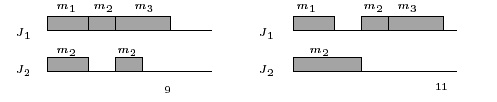
\includegraphics[width=7cm]{./figures/scheduling.jpg}
	\caption{Schedules for jobshop example (with makespan 9 (left) and 11 (right)) \cite{AM02}}
	\label{fig:schedules_maler}
\end{figure}
%%%\subsection*{Geometrical Representation of $\Ko$}\label{app:geom}

\begin{figure}[ht!]
	\centering
 		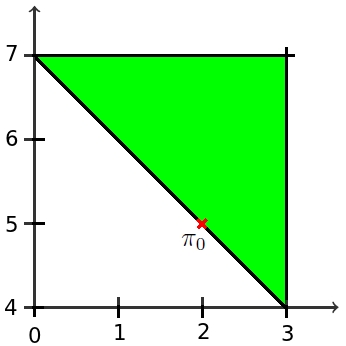
\includegraphics[width=3cm]{./figures/geom.jpg}
	\caption{Geometrical representation of $\Ko$ around $\pio: (2,5)$.}
	\label{fig:geom}
\end{figure}

%%%%\subsection*{Example of Trace Set (Jobshop example of \cite{AM02})}\label{app:traceset}
%-%-%-%-%-%-%-%-%-%-%-%-%-%-%-%-%-%-%-%-%-%-%-%-%-%-%-%-%-%-%
\begin{figure}[ht!]
	\centering
 		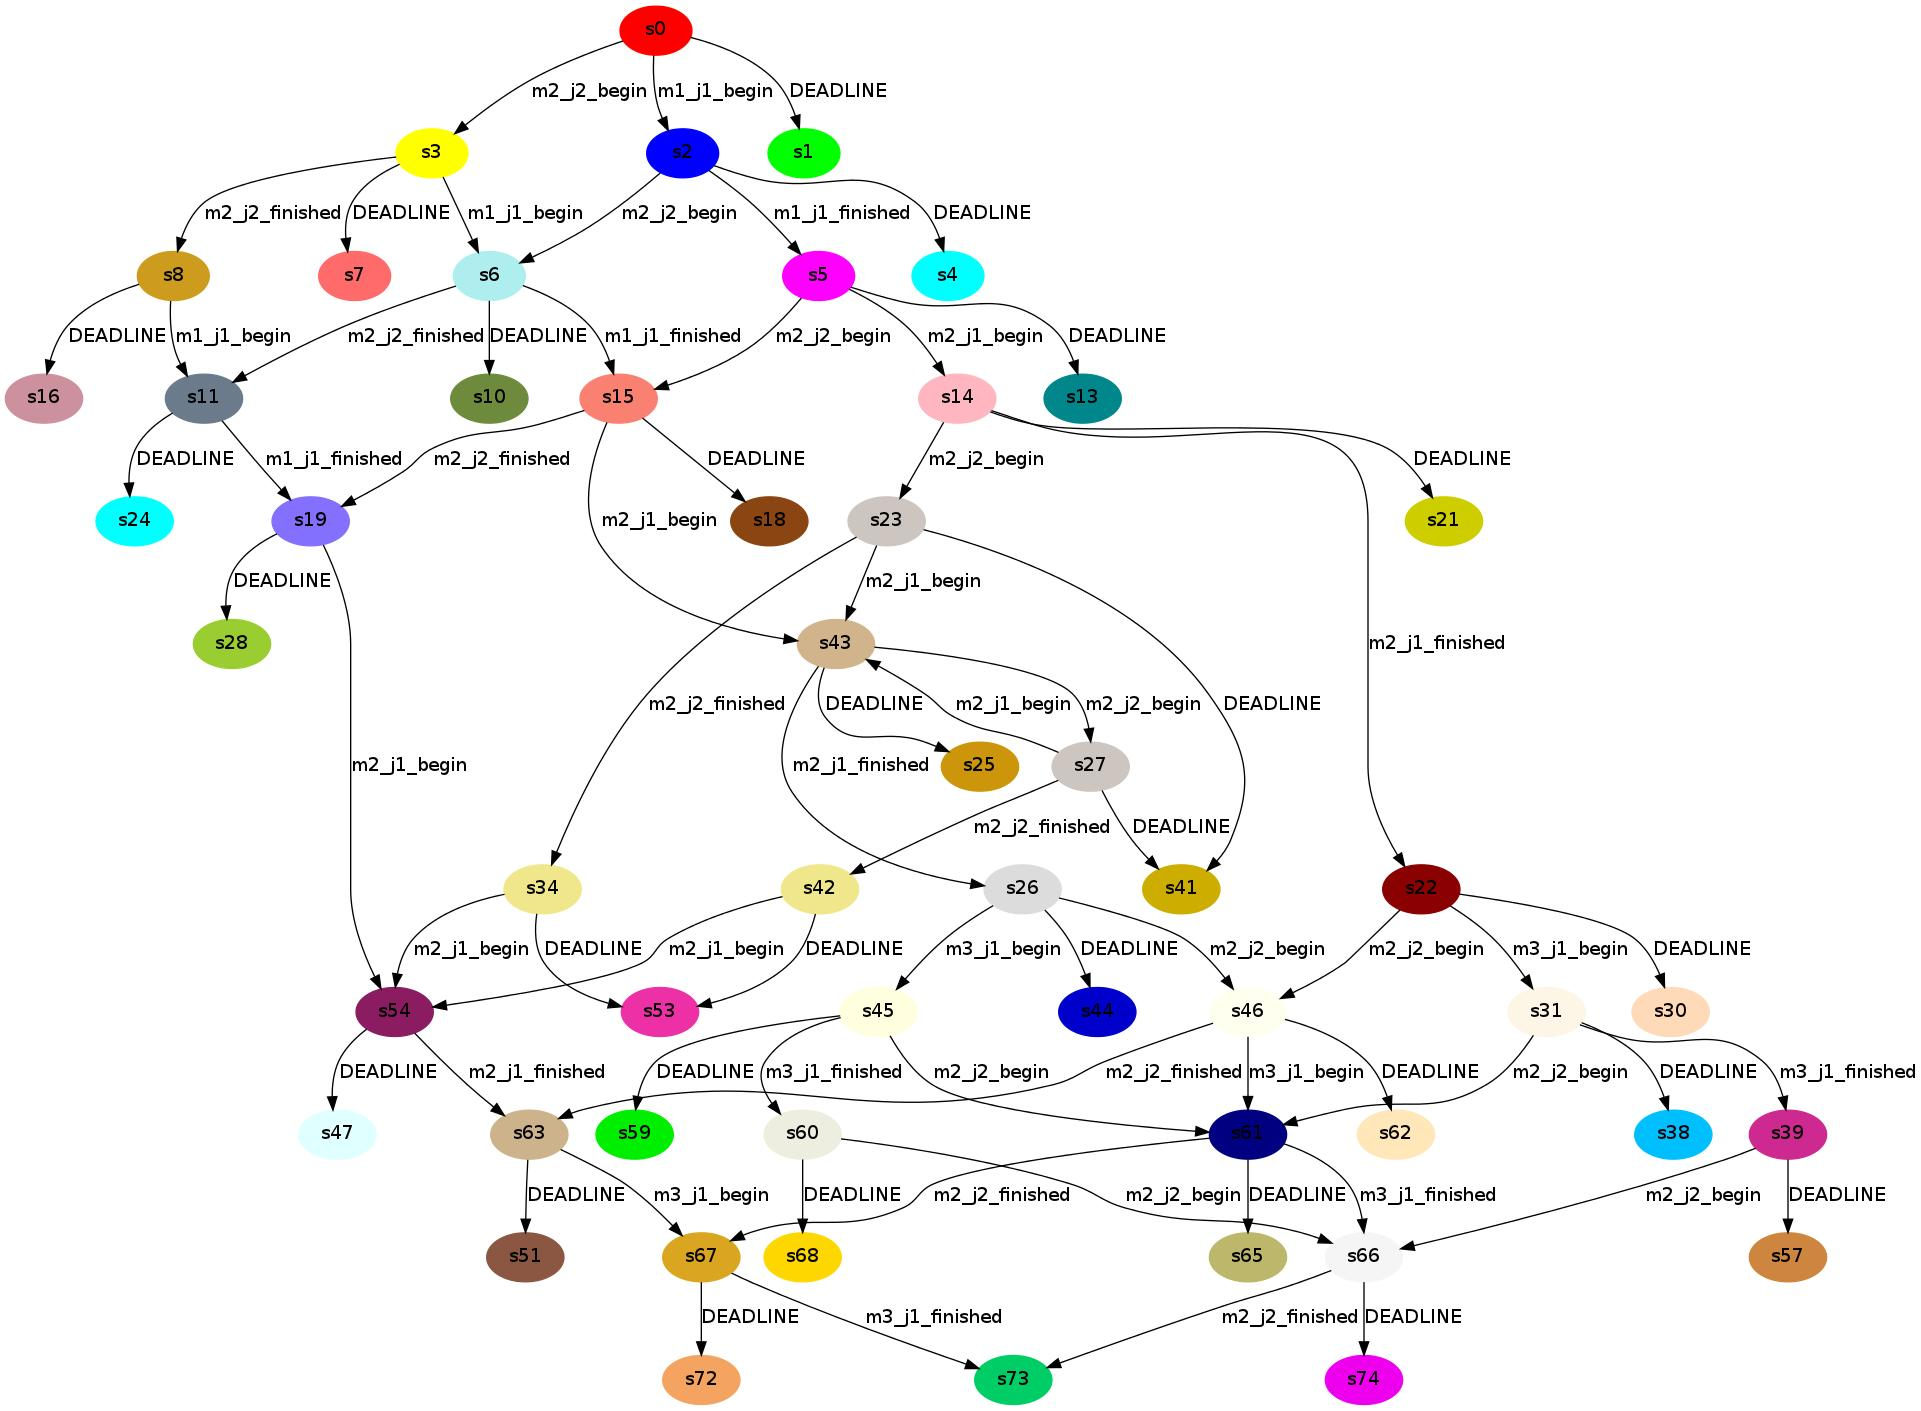
\includegraphics[width=10cm]{./figures/traceset.jpg}
% 	\commentaire{TO DO}
	\caption{Graphics of the trace set output by \imitator{} on the jobshop example}
	\label{fig:output}
\end{figure}
%-%-%-%-%-%-%-%-%-%-%-%-%-%-%-%-%-%-%-%-%-%-%-%-%-%-%-%-%-%-%
%%%%%%



%\commentaire{commenter figure: maler, merging; seul l'etat du bas respecte}
%\commentaire{
%un automate par tache, un scheduler
%}
%\commentaire{
%ex de TA en appendix, avec schema et code IMITATOR
%}

\section*{Appendix 2: Rate Monotonic Case Study from \cite{bb04}}
\label{app:carto}
We present here what we can obtain from \imitator{} 2.5 with the Behavioral Cartography ($\BC$) output. By iterating $\IM$ over all the integers points %(or each step given by a rational value, e.g., $1/3$)
inside a finite but dense rectangle $V_0$ in the parametric space, one is able to decompose (most of) the parametric space included into $V_0$ into behavioral tiles\footnote{Actually, one can take a finer discretization step than integers to ensure a better coverability of~$V_0$}~\cite{af10}.

For a given tile, we ensure that for every valuation of the parameters in this tile, the behavior of $\A$ is the same;
therefore, we only have to test the schedulability of a single point for each tile to ensure the schedulability on the whole tile.

Let us apply this method on a ``Rate monotonic'' example of \cite[Section~III]{bb04}.
There are three periodic tasks $\tau_1, \tau_2$ and $\tau_3$ with periods of $T_1 = 3, \ T_2 = 8$ and $T_3 = 20$ and deadlines of $D_1 = 3, \ D_2 = 8$ and $D_3 = 20$.
We are interested in finding the set of computation times of each task such that the system is schedulable.
(The interested reader can find the full details in \cite{bb04}.)

We set $V_0$ as $C_1 \in [0,3]$, $C_2 \in [0,8]$ and $C_3 = 0$, where $C_i$ is the computational time of $\tau_i$. The system is unschedulable if there exists a task $\tau_i$ such that $C_i > T_i$. 
% We recall the algorithm for $\BC$, we first pick an integer point $\pi_k$ that does not belong to any tile already computed and we synthesize $\IM(\A,\pi_k)$ which will be a new tile. We iterate this process 
% until no integer point remains uncover (since $V_0$ only contains a finite number of integer points, we know that GC will terminate in a finite number of iterations).
Algorithm~$\BC$ outputs the set of tiles and we check for one point of each tile whether the system is schedulable or not.
The result for this example is given in Figure \ref{fig:carto} for this $V_0$ with a discretization step of $0.2$.

\begin{figure}[!ht]
	\centering
	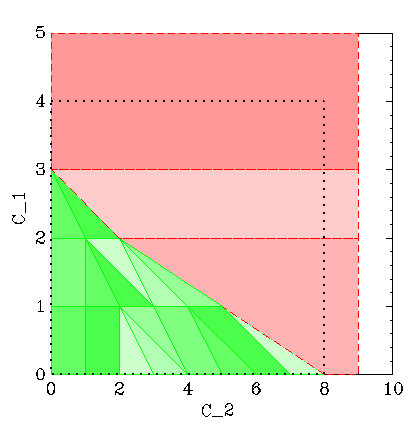
\includegraphics[scale = 0.5]{./figures/C1-C2.png}
	\caption{Cartography output by \imitator{} 2.5 (in green the system is schedulable; in red, unschedulable)}
	\label{fig:carto}
\end{figure}

Note that the full dense parametric space (including beyond~$V_0$) is covered after only 20 applications of~$\IM$.
The green part corresponds to the bottom left ``triangle'' of~\cite[Figure~1(a)]{bb04}.


% 
% \subsection*{Summary of Experiments}
% 
% %\commentaire{ajouter un beau tableau avec des contraintes, et un lien vers un rapport d'etudes de cas (+ site Web)}
% 
% \begin{table}[!ht]
%  \centering
% \begin{tabular}{|c|c|c|c|c|c|c|c|c|}
% \hline
%  Case study             & $|\mathcal{A}|$& $|X|$ & $|P|$ & $|S|$        & $|T|$         & $n$   &
% $|K|$ & t               \\
% \hline
% jobshop $2\times 3$ \cite{AM02}               & 4 & 6         & 8     & 676/3194      & 886/3931      & 15/15 & 15/10
% & 288.2/450.4   \\
% \hline
% jobshop $2\times 5$               & 4 & 6         & 8     & 676/3194      & 886/3931      & 15/15 & 15/10
% & 288.2/450.4   \\
% \hline
% jobshop $3\times 5$               & 4 & 6         & 8     & 676/3194      & 886/3931      & 15/15 & 15/10
% & 288.2/450.4   \\
% \hline
% cpr08 \cite{cpr08}               & 4 & 6         & 8     & 676/3194      & 886/3931      & 15/15 & 15/10
% & 288.2/450.4   \\
% \hline
% hppr10 \cite{LPPRC10}             & 3 & 4 &  9& 60/103    & 103/686               & 10/10 & 7/5 &
% 2.10/11.7\\
% \hline
% Task chains \cite{SGL97} & 8 & 15 & 18 & 215/1364 & 264/1363 & 15/15 &
% 17/17 & 85.3/270.6\\
% \hline
% %Astrium (RM) \cite{soulat12}       & 5 & 7         & 10    & 63/63         & 62/62         & 32/32 &
% %12/12 & 1.10/0.93       \\
% %\hline
% RM 1            & 5 & 7         & 10    & 205/805       & 225/837       & 40/40 & 11/11 & 15.6/28.5  \\
% \hline
% RM 2            & 5 & 7         & 10    & 208/1174      & 228/1269      & 42/42 & 12/12 & 10.7/41.0  \\
% \hline
% RM 3            & 5 & 7         & 10    & 49/82         & 51/81         & 15/15 & 12/12 & 1.03/1.75  \\
% \hline
% %Astrium (EDF)   & 5 & 10        & 13    & 63/63         & 62/62         & 32/32 & 13/13 &
% %2.42/2.30       \\
% %\hline
% EDF 1           & 5 & 10        & 13    & 76/415        & 91/454 & 31/31        & 20/20 & 66.1/288.2  \\
% \hline
% EDF 2           & 5 & 10        & 13    & 254/642       & 326/817       & 47/47 & 12/12 & 9.9/23.2  \\
% \hline
% EDF 3           & 5 & 10&  13   & 31/43         & 33/45         & 9/9   & 13/14 & 1.09/1.57  \\
% \hline
% \end{tabular}
% \caption{Experimental results with \imitator{} on scheduling examples}
%  \label{table:results}
% \end{table}
% 
% 
% 
% \commentaire{
% quand il y a une variablité du computation time (entre BCET et WCET), pas de méthode exacte analytique --> interet des methodes symboliques (model checking) d'exploration exhaustive basee sur TA (et donc interet de IM puisque generalisation! si on etait schedulable, on lest encore avec IM)
% }
% 
% Astrium, RMs and EDFs case studies are composed of three cyclic tasks that need to be performed on a single machine.
% 	Therefore, the machine has to choose which task is active when several tasks are requiring computation.
% 	This is done in two ways, either with a Fixed Priority (RM) scheduler or an Earliest Deadline First scheduler (EDF).
% 	These three case studies are being studied in the framework of the joint project Roscov between LSV and Astrium.
% 	
% cpr08~\cite{cpr08} and HPPR10~\cite{LPPRC10} are two-cyclic-tasks problem with an EDF scheduler.
% 	TaskChain~\cite{SGL97} does not use cyclic tasks but instead has a 4 task chain and a concurrent 3 task chain.
% 		Each task in a chain cannot start until the previous one has not terminated.
% 		Each task in each chain has a given fixed priority.
% 		A scheduler assigns which task has the computational time with a RM policy.
% 
% For every RM scheduling example, the parameters are the offsets of the tasks, their Wost Case Execution Time (WCET), their periods and a deadline to achieve a given goal (modeled by an extra automaton).
% 	For every EDF scheduling example, the parameters are the offsets of the tasks, their WCET, their periods, a deadline to achieve each task and a deadline to achieve a given goal (modeled by an extra automaton).
% 
% 
% 
% Experiments were performed on Ubuntu 11.10 equipped with an Intel Core\,2 2.93\,GiHz processor with 2\,GiB RAM.
% Source code, binaries, all case studies and logs are available in
% \url{http://www.lsv.ens-cachan.fr/Software/imitator/}.
% 
% All case studies and experiments are also described in a research report~\cite{soulat12}.
% 
% 
% %\subsection*{Example of Trace Set}
% 
% %\commentaire{ajouter un trace set en mode fancy}
% 
% %\subsection*{An Example of Model}
% 
% %\commentaire{ajouter un modele en entree avec sa representation graphique (pour decrire la syntaxe)}

\end{document}     